\chapter{Návrh riešenia}
Východiskom pre riešenie spracovania akceleračných dát budú nasledujúce výskumné otázky, ktoré
sa pokúsime zodpovedať za kontrolovaných aj reálnych podmienok primárne na vlastných datasetoch:

\begin{itemize}[noitemsep]
	\item Ako vplýva nastavenie parametrov metód časovej a frekvenčnej analýzy na úspešnosť detekcie význačných udalostí,
	teda náhlych zmien distribúcie v čase a hlavných frekvenčných komponentov?
	\item Aká úspora v množstve prenášaných dát sa dosiahne rozličnými technikami na sumarizáciu vzoriek?
	\item Aká je výpočtová náročnosť a časť odozvy spôsobov detekcie udalostí?
	\item Aká je presnosť odhadu rýchlosti a polohy z akcelerácie?
	\item Aká syntax pravidiel môže byť vhodná na vzdialenú konfiguráciu dátovej pipeline IoT zariadenia?
	\item Ktorý bezdrôtový komunikačný protokol postačuje pre implementované modely spracovania?
\end{itemize}

Navrhované zariadenie bude postavené na platforme mikrokontroléra ESP32 od Espressif, pretože pri nízkej
obstarávacej cene ponúka možnosť konektivity s Wifi a Bluetooth a v porovnaní s podobnými zariadeniami dostatočný
výpočtový výkon a kapacitu pamätí, čo ho činí vhodný na experimentovanie. Diagram aktivít na obr. \ref{fig:design}
vizualizuje navrhovaný beh činností na zariadení.

Po zapnutí sa začne čítanie vzoriek z akcelerometra s nastaveným dynamickým rozsahom, nad určitú
prahovú úroveň amplitúdy a so vzorkovacou frekvenciou podľa ODR. Podľa pravidlami aktivovanými modulmi bude
súbežne vykonateľných 5 ciest spracovania.

Frekvenčná analýza bude pozostávať z krokov oknovania signálu  zvoliteľnou oknovou funkciou nastaviteľnej veľkosti,
následne sa signál transformuje do frekvenčnej domény,
kde dôjde k vyhladeniu spektra kĺzavým priemerom alebo Welchovou metódou a nakoniec sa podľa prítomnosti špičiek
vo frekvenčnom vedierku vytvorí udalosť na začiatku a na konci súvislého časového pôsobenia. Časová analýza
bude detegovať náhle zmeny v priebehu signálu na základe štatistík polohy, rozptýlenosti a tvaru
distribúcie vzhľadom na predošlé okná. Okrem toho sa môžu po podvzorkovaní odosielať alebo ukladať ,,surové dáta''
hodnôt veličiny v čase alebo frekvenčných vedierok. Numerická kvadratúra korigovaná obálkami umožní extrahovať zo
snímaného zrýchlenia odhad o rýchlosti a polohe.

\begin{figure}[h]
	\centering
	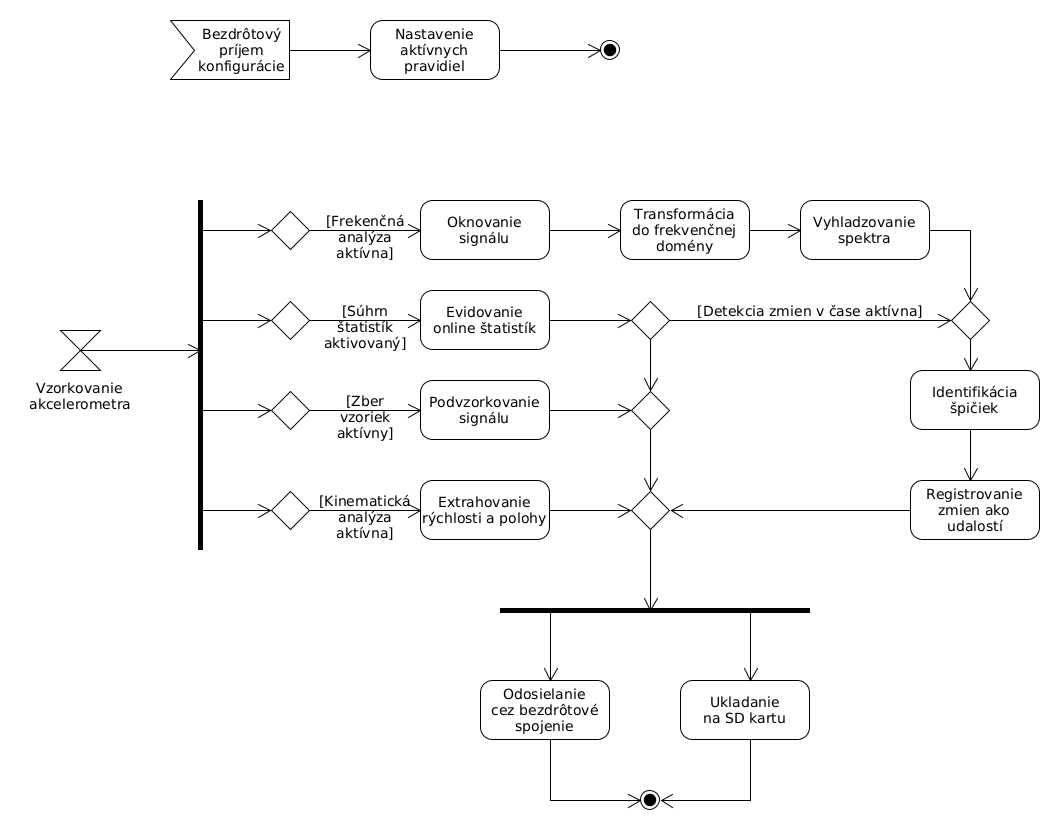
\includegraphics[width=\textwidth]{figures/design.png}
	\caption{Diagram aktivít navrhovaného systému na spracovanie dát zo senzora}
	\label{fig:design}
\end{figure}

\emptypage
